\chapter{Stand der Technik}
\section{Akkusysteme}
Verschiedene Speicher für elektrische Energie, die auf einer elektrochemischen Basis basieren, nennt man Batterien oder auch Akkumulatoren. Elektrochemische Speicher haben in den vergangenen Jahren immer mehr an Bedeutung gewonnen und werden auch in Zukunft immer öfter Gebrauch finden. Möglich wurde unsere heutige elektronische Mobilität erst mit der Erfindung der galvanischen Zelle. Seit dieser Erfindung,die mit Hilfe eines Stromkreises chemische Energie in elektrische Energie umzuwandelt, hat sich über die jahrzentelange Weiterentwicklung der Batterie einiges getan. Die Einsatzmöglichkeiten von Akkumulatoren sind extrem vielfältig. Kleine Lithium-Ionen Akkus werden zum Beispiel als Knopfzellen in Smartphones verwendet. Jedoch können sie auch bis hin zu großen stationären Energiespeichern für erneuerbare Energien benutzt werden. Wie bereits vorher erwähnt, sind elektrische Energiespeicher ein wichtiger Bestandteil für den Erfolg der Elektromobilität geworden. Es gibt unzählig viele verschiedene Arten von Batterien, die sich im chemischen Aufbau, ihrer Form und natürlich in ihren Einsatzmöglichkeiten unterscheiden. Durch die äußerst besonderen chemischen Eigenschaften und die vielseitigen Anwendungsbereiche, hat sich der Lithium-Ionen Akku durchgesetzt.
\newpage

\section{Batteriearten}

\subsection{Bleiakkumulator}
Die ersten Versuche, einen auf Blei basierenden Akkumulator zu entwickeln, wurden am Anfang des 19. Jahrhunderts durchgeführt. Industriell wurde der Bleiakku interessant, als Forscher und Chemiker zusammen 1880 ein Verfahren entwickelten, bei dem der Bleiakkumulator bereits nach wenigen Ladezyklen, eine hohe Kapazität erreichte. Der erste technisch einsetzbare Bleiakkumulator wurde 1886 von Henri Tudor entwickelt. Dieser besitzt eine Zellspannung von ungefähr 2V (abhängig vom Ladezustand), was eine durchaus große Spannung für sogenannte "wässrige Syteme"  ist. Der Ausdruck "wässrige Systeme"  leitet sich von dem Elektrolyt ab. Bei Bleiakkumulatoren wird wässrige Schwefelsäure als Elektrolyt verwendet. Im entladenen Zusatnd bestehen beide Pole aus Blei(II)-sulfat (PbSO4). Weiters besteht die Kathode aus Blei und die Anode aus Bleioxid. Bleiakkumulatoren sollten keinesfalls tiefenentladen werden, da dies zu Schäden führt und den Akku unbrauchbar macht. Ein extrem großer Nachteil ist das Gewicht, da nur 30 bis 40Wh/kg erreicht werden können.
Diese Art von Akku zeichnet sich durch das kurzzeitige Zulassen hoher Ströme aus die zum Beispiel für Fahrzeug -bzw. Starterbatterien notwendig sind. Unter anderem sind 50 Prozent des Batteriemarkets von Bleiakkumulatoren belegt. Wie vorher bereits erwähnt werden diese oftmals in Autos, LKWs oder auch Motorräder verbaut.

\subsection{Nickel-Metallhybrid Akkumulatoren}
Die technischen Grundlagen des Nickel-Metallhybrid Akkumulator wurden von Stanford R. Ovshinsky und Masahiko Oshitani ab 1962 bis 1982 zur marktreifen Zelle entwickelt. Seit dem Jahr 2006 sind spezielle NiMH-Akkumulatoren auf dem Markt, die sich gegenüber herkömmlichen NiMH-Akkus durch eine deutlich reduzierte Selbstentladung auszeichnen. Die positive Elektrode eines Nickel-Metallhybrid Akkumulators(NiMH) besteht aus Nickel(II)-hydroxid wogegen sich die negative Elektrode aus einem Metallhybrid zusammensetzt. Als Elektorlyt verwendet dieser Akkumulator eine Wasserstoffspeicherlegierung aus Nickel und seltenen Erden. NiMH-Akkus erreichen bis zu 80Wh/kg. Sie sind vielfach in den üblichen Bauformen von Standardbatterien verbreitet und liefern pro Zelle eine Spannung von 1,2V. Oftmals werden sie als wiederaufladbare Alternative der gängigen Alkalibatterien in haushaltsüblichen Geräten eingesetzt. Ein großer Vorteil gegenüber den Nickel-Cadmium Batterien ist es, das der NiMH Akku nicht aus giftigen Cadmium besteht und er außerdem eine höher Energiedichte aufweist.
Der Anwendungsbereich von NiMH Akkumalatoren ist sehr vielfältig. Vorzugsweise kommen sie wie NiCd Akkus überall dort zur Anwendung, wo ein hoher Energiebedarf besteht und hohe Batteriekosten vermeiden werden sollten. Tyische Anwendungsbereich sind zum Beispiel Foto- Videogeräte, Elektroautos, Elektrowerkzeuge und noch viele mehr. NiMH Akkus werden außerdem oft als Energiespeicher für Notbeleutungsanlagen verwendet.
\newpage
\subsection{Nickel-Cadmium Akkumulatoren}
1899 wurde der Nickel-Cadmium Akku von dem Schweden W. Jungner entwickelt. NiCd Akkus zeichnen sich dadurch aus, dass sie einen eingebauten Ent- und Überladeschutz integriert haben. Das hat zur Folge, dass man keine aufwendige elektronische Beschaltung durchführen muss. Als Material für die Kathode dieses Akkus verwendet man Nickeloxidhydroxid. Die Anode dagegen besteht aus dem giftigen Material Cadmium, welches jedoch eine äußerst hohe spezifische Ladung (478Ah/kg) besitzt. Bei Nickel-Cadmium Akkumulatoren besteht das Elektorlyt aus Kalilauge. Die typische Nennspannung ist exakt die selbe wie bei NiMH Akkus, 1,2V. Aus dieser Zellenspannung ergibt sich eine spezifische Energie von ungefähr 60Wh/kg. Eine Eigenschaft die man bei anderen Technologien nur selten antrifft ist das hervorragende Tieftemperaturverhalten von NiCd Akkus. Selbst bei einer Temperatur von -40°C ist eine Inbetriebnahme noch möglich. Im Jahr 2004 wurde jedoch die Verwendung von Nickel-Cadmium Akkus wegen dem giftigen Material auf medizinische und sicherheitrelevante Bereiche begrenzt. Diese Akkumulatoren sind in 2 verschiedenen Bauformen verfügbar, die sich durch die unterschiedlichen Anwendungsbereiche unterscheiden. Die offene Bauweise wird meist für Starterbatterien für Verbrennungsmotoren und Traktionsbatterien für Elektrofahrzeuge verwendet. Bei der anderen Bauweise, werden die Zellen gasdicht verschlossen. Oftmals werden sich für zentrale Stromversorgungssysteme für Notbeleuchtung verwendet.
\newpage

\subsection{Lithium-Ionen Batterie}
\subsubsection{Geschichte}
Schon bereits in dem Jahr 1970 wurde von Jürgen Otto Besenhard und anderen das grundlegende Funktionsprinzip der Alkalimetallionen-Interkalation in Kohlenstoff-Elektroden sowie auch in oxidischen Elektroden erforscht und veröffentlicht. Ebenfalls wurde dabei die Anwendung in Lithium Batterien untersucht auch wenn zu der Zeit die praktische Anwendbarkeit als Elektroden für Lithium Batterien noch nicht erkannt wurde. Der erste auf dem Markt erhältliche Lithium-Ionen Akkumulator wurde von Sony im Jahr 1991 angeboten. Dieser Lithium-Cobaltdioxid Akku wurde in einer Videokamera verbaut. Die Batterie, die eine Spannung von 7,2V aufweiste, bestand aus zwei seriell verschalteten Zellen und weiste etwa eine Kapazität von 1200mAh auf. Sogar bis heute wird diese Bauform von Akkumulatoren mit Kapazitäten
bis zu 6900mAh angeboten und in äußerst vielen Geräten eingesetzt. Drei Physiker bzw. Chemiker (Whittingham, Goodenough und Yoshino) erhielten 2019 sogar den Nobelpreis für Chemie, für die Entwicklung der Lithium-Ionen Batterie.
Forscher einer Universität fanden im Jahr 2020 heraus, dass durch die Zugabe von dem Element Kalium die Lithium Akkumulatoren langlebiger und sicherer werden. Außderdem verhindert das Kalium in dem Akku unerwünschte chemische Nebenreaktionen.
\subsubsection{Allgemeines}
Es gibt zahlreiche verschiedene Bauformen von Lithium-Ionen Akkumulatoren. Diese Batterien unterscheiden sich nicht nur in ihrer Größe und der Bauform, sondern auch in der chemischen Zusammensetzung ihrer Komponenten und haben unter anderem auch verschiedene Spannungsbereiche. Kenndaten wie Zellenspannung, Lade- und Entladeschlussspannung, Temperaturempfindlichkeit und der maximal zulässige Lade- oder Entladestrom variieren bauartbedingt und sind wesentlich vom eingesetzten Elektrodenmaterial und den Elektorlyten abhängig. Eine Eigenschaft die alle Lithium-Ionen Akkumulatoren gemeinsamen haben ist, dass sie gasdicht versiegelt sein müssen und außerdem lageunabhängig betrieben werden können. Die spezifische Energiedichte liegt ungefähr in der Größenordnung von 150Wh/kg und weist eine Energiedichte von 400Wh/l auf. Durch diese Eigenschaften findet diese Art von Batterie besonderen Einsatz in der mobilen Branche als elektrischer Energiespeicher. Ein weiteres wichtiges Merkmal aller Lithium-Ionen Akkumulatoren ist, dass sie Überladungen nicht verkraften können. Wenn man mehrere Zellen zum Beispiel in Reihe schaltet, um eine höhere elektrische Spannung zu erzielen, müssen zum Ausgleichen der Toleranzen in der Kapazität zwischen den Zellen meistens zusätzlich ein Batteriemanagementsystem (BMS) und ein Balancer vorgesehen werden.  
\newpage

\subsubsection{Prinzip der Lithium-Ionen Batterie}
Ein Lithium-Ionen Akkumulator erzeugt durch die Verschiebung von Lithium-Ionen eine elektromotorische Kraft.
Beim Ladevorgang wandern positiv geladene Lithium-Ionen durch einen Elektrolyten hindurch von der positiven Elektrode zur negativen, während der Ladestrom die Elektronen über den äußeren Stromkreis liefert. Eine negative Elektrode aus Lithium-Metall ist elektrochemisch optimal, für einen Akku aber ungeeignet. Da sich die Elektrode beim Entladevorgang genauso wie bei einer Lithium-Batterie auflöst, besteht beim Ladevorgang keine Möglichkeit mehr, ihre Geometrie zu rekonstruieren.

\textbf{Aufbau:}

Die negative Elektrode eines gänigen Lithium-Ionen Akkus besteht meist aus Graphit. Die positive Elektrode hingegen enthält meist Lithium-Metalloxide in Schichtstruktur wie Lithiumcobaltoxid (LiCoO2). Der Lithium-Ionen Akkumulator muss wasserdicht sein, da es sont zu einer Nebenreaktion zwischen dem Wasser (H2O) mit dem Leitsalz (LiPF6) zu Flusssäure (HF) reagieren kann. Das am häufigsten verwendete Elektrolyt in Lithium-Ionen Akkumulatoren besteht aus einer Mischung zwischen wasserfreien Lösungsmitteln (Ethylencarbonat, Propylencarbonat) mit Alkylcarbonaten/Äthern (Dimethylcarbonat, Diethylcarbonat) und natürlich mit Lithiumsalzen.

Beim Aufladen der Lithium-Ionen Akkus, d.h. anlegen einer äußeren Potenzials, fließen Lithium-Ionen zwischen die Graphitebenen (nC). Zusammen mit dem Kohlenstoff bilden diese Ionen eine Interkalationsverbindung (LixnC). 
Anders als beim Aufladen, wandern die Lithium-Ionen beim Entladen wieder in das Metalloxid und die Elektronen der Batterie können über einen äußeren Stromkreis wieder zur positiven Elektrode fließen. 
Ausschlaggebend für diese Interkalationsverbindung ist die Ausbildung einer schützenden Deckschicht auf der neagtiven Elektrode. Für die Lithium-Ionen ist diese Schicht durchlässig, jedoch die Lösungsmittelmoleküle können diese Deckschicht nicht durchdringen. Es kann passieren, dass diese Deckschicht nicht genügend ausgebildet worden ist. Das hat zur Folge, dass die Lithium-Ionen mit den Lösungsmittelmolekühlen interkalieren, wodurch die Graphitelektrode stark beschädigt, oder sogar zerstört wird.

\textbf{Reaktionsgleichungen:}
\begin{itemize}
	\item \textbf{Negative Elektrode (Entladung):} \medskip\\
	LiCn  -->  nC + xLi+ + xe-

	\item \textbf{Positive Elektrode (Entladung):}\medskip\\
	LiMn2O4 + xLi+ + xe-  -->  LiMn2O4

	\item \textbf{Redox Gleichung:}\medskip\\
	LiMn2O4 + LiCn  -->  LiMn2O4 + nC
\end{itemize}

\begin{figure}[H]
	\begin{center}
		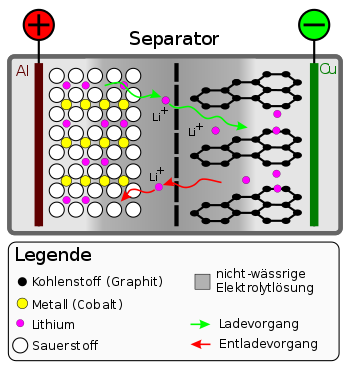
\includegraphics[scale=0.5]{figures/Akku/350px-Li-Ion-Zelle_(CoO2-Carbon,_Schema).svg.png}
		\caption{Grundaufbau einer Lithium-Ionen Zelle}
	\end{center}
\end{figure}
\newpage

\subsubsection{Lagerung und Sicherheithinweise}
Auch wenn Lithium nur als Li-Verbindungen in Lithium-Ionen Akkumualtoren vorhanden sind, sind die Komponenten eines solchen Akkus extrem leicht entzündbar, da Lithium ein hochreaktives Metall ist. Beim Überladen sind Ausgleichsreaktionen (z.B. die Zersetzung von Wasser), bei Lithium-Ionen Akkus nicht möglich, wie bei anderen Akkumualtoren dies der Fall ist. Schutzschaltungen die intern verbaut sein sollten, müssen eine solche Verpufferung verhindern. Anderfalls wird sonst die Funktionsfähigkeit des Akkus zerstört und er wird unbrauchbar. 
Jedoch kann es nicht nur zu inneren Beschädigungen kommen. Im Falle von inneren Kurzschlüssen, kann es passieren, dass mechanische Beschädigungen entstehen. Der hohe Kurzschlussstrom lässt zum Beispiel das Gehäuse schmelzen oder sogar in Flammen aufgehen. Es kann auch passieren, dass man den Defekt nicht unmittelbar erkennen kann. Doch kurze Zeit später kann es bereits zum Ausbruch eines Feuers kommen.

\textbf{Lagerung:}

Im Idealfall, sollten Lithium Ionen Akkus bei einem Ladezustand zwischen 40 - 60 Prozent kühl aufbewahrt und gelagert werden.


\textbf{Sicherheitshinweise:}

\begin{itemize}
	\item{Es ist wichtig, dass Lithium-Ionen Akkus nur mit passenden Ladegeräten aufgeladen werden. Schnell-Ladegeräte für Lithium Akkumulatoren können beispielweise eingesetzt werden. Man muss darauf achten, dass sie immer unter Aufsicht und möglichst nicht in der Nähe von brennbaren Materialien benutzt werden.} \medskip\\

	\item {Lithium-Ionen Akkus sind zwar hermetisch gekapselt, dennoch sollten sie unter keinen Umständen in Wasser getaucht werden. Besonders defekte und  vollgelade Lithium-Zellen reagieren meist heftig mit Wasser.}\medskip\\
	
	\item {Lithium-Ionen Akkumulatoren sind mechanisch sehr empfindlich. Durch einen internen Kurzschluss und einem Kontakt mit Luft können sie sich schnell entzünden.}\medskip\\
	
	\item {Eine Lithium-Ionen Zelle die in Flammen steht, wenn möglich mit Sand und nicht mit Wasser löschen, da dies zu einer heftigen Reaktion führen kann.}\medskip\\
	
	\item {Lithium-Zellen sollten niemals über 4,2V geladen und nicht unter 2,5V pro Zelle entladen werden. Außerdem dürfen Zellen niemals kurzgeschlossen werden. Bei einem Ladvorgang ist auf eine gute Wärmeabfuhr zu achten (nicht in die Sonne legen).}\medskip\\
	
	\item {Mehrere Lithium-Zellen sollten nur dann gleichzeitig geladen werden, wenn eine Schutzschaltung vorhanden ist.}\medskip\\
	
	\item {Die Elektorlytflüssigkeit ist brennbar. Sollte aus einer Zelle Elektrolytflüssigkeit austreten, diese am besten sofort ordnungsgerecht entsorgen.}\medskip\\
	
	\item {Man sollte versuchen die Lithium-Zellen bei einer Restkapazität von 20 Prozent nachzuladen.}\medskip\\

\end{itemize}
\newpage

\subsubsection{Anwendungbereiche von Lithium-Ionen Akkumulatoren}
Lithium-Ionen Akkus versorgten anfangs hauptsächlich tragbare Geräte mit hohem Energiebedarf, für die herkömmliche Nickel-Cadmium- oder Nickel-Metallhydrid Akkus zu schwer oder zu groß waren, beispielsweise Mobiltelefone, Tablets, Digitalkameras, Camcorder, Notebooks, Handheld-Konsolen oder Taschenlampen. In der heutigen Zeit sind Lithium-Ionen Akkumulatoren fast in allen denkbaren Bereichen aufzufinden. In der Elektromobiliätsbranche dienen sie oftmals als Energiespeicher für Elektroautos, moderne elektronisch betriebene Rollstühle und auch für Hybridfahrzeuge. Auch im Modellbau haben sie schon früh Verwendung gefunden. Dadurch, dass Lithium Akkus ein deutlich geringeres Gewicht als andere Batteriearten aufweisen, sind sie in Verbindung mit bürstenlosen Gleichstrommotoren und den entsprechenden Reglern, gut als Antriebseinheit im Flugmodellbau geeignet. Scho seit Anfang des 21. Jahrhunderts, gibt es Lithium-Ionen Akkus auch in Elektrowerkzeugen wie zum Beispiel Akkuschraubern. Auch im Flugbetrieb haben diese Batterien Verwendung gefunden. In der Boeing 787 werden ebenfalls Lithium-Kobaltoxid-Akkus (LiCoO2) verwendet. Zum Großen Teil werden Lithium-Ionen-Batterie-Systeme auch in Batterie-Speicherkraftwerken und Solarbatterien eingesetzt.
\newpage


\subsection{Batteriemanagementsystem}
Batteriemanagementsysteme (BMS) sind elektronische Regelschaltungen, die Akkumulatoren oder Akkupacks auf Ladung und Entladung überwachen und ebenfalls regeln. Die Batteriekennwerte die man überwachen kann bzw. möchte, hängen oftmals von dem Projekt ab. Zu den häufigsten Batteriekennwerten gehören die Erkennung des Batterietyps, die Batteriespannung, die Spannung sowie die Temperatur einzelner Batteriezellen, die Akkukapazität, der Ladzusatnd, die Restbetriebszeit, die Stromentnahme und einige Kennwerte mehr. Die Hauptaufgabe von BMS-Systemen besteht darin, sicherzustellen, dass die Restenergie in einer Zelle optimal genutzt wird. Um keine Beschädigungen an Zellen zu bekommen, schützt das Batteriemanagementsystem die Batterien vor Tiefenentladung, vor Überspannung, vor zu schneller Ladung (begrenzen des Ladestroms) und ebenfalls vor einem zu hohen Entladestrom. Bei Akkupacks, d.h. Akkumulatoren mit mehreren Zellen, sorgt das Batteriemanagementsystem außerdem für ein sogenanntes Balancing, das sich darin ausdrückt, dass die verschiedenen Batteriezellen gleiche Ladezustände und Entladezustände haben.

\begin{figure}[H]
	\begin{center}
		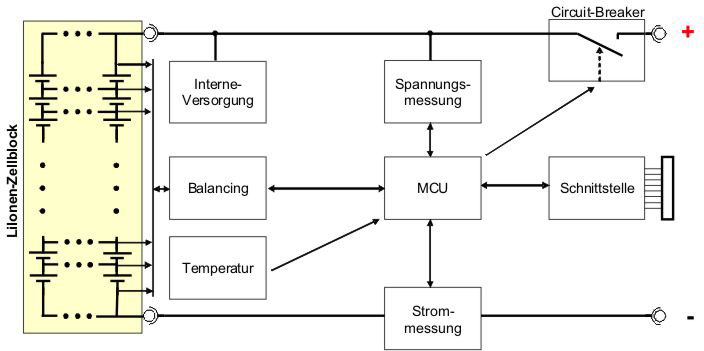
\includegraphics[scale=0.5]{figures/Akku/bms-1schaltunggrund.jpg}
		\caption{Grundschaltung eines Batteriemanagementsystems}
	\end{center}
\end{figure}

Grundsätzlich setzt sich ein vollständiges Batteriemanagementsystem aus folgenden Komponenten zusammen:
\begin{itemize}
	\item \textbf{Cell Supervising Circuit(CSC):} \medskip\\
	Die Aufgabe des CSC besteht darin die Zellen auf Spannung und 			Temperatur zu überwachen.

	\item \textbf{Kontrolleinheit:}\medskip\\
	Die Kontrolleinheit berechnet die State of Charge (SOC), die State 	of Health (SOH) und überprüft auch die Funktionalität der 				Batterien (State of Function). Außerdem wird von der 					Kontrolleinheit auch der Ladeausgleich gesteuert und kommuniziert 		über eine Serielle Schnittstelle mit einem Prozessor. 

	\item \textbf{Circuit Breaker:}\medskip\\
	Der Circuit Breaker trennt im Fehlerfall die Batterie von der 			Last. Dies erfolgt mithilfe eines HS-Kontaktors.
	
	\item \textbf{Strommessvorrichtung:}\medskip\\
	Diese Komponente ist für die Messung des Stromes zuständig.
	
	\item \textbf{Temperaturüberwachung:}\medskip\\
	Diese Komponente überprüft, ob sich die Batterien oder die 				Akkupacks in einem zulässigen Temperaturbereich befinden.
\end{itemize}
\newpage

\subsubsection{Komponenten eines BMS}

\textbf{Cell Supervising Circuit (CSC):}
Die erste Komponente eines Batteriemanagementsystem ist für die Spannungs- und Temperaturüberwachung der einzelnen Zellen zuständig und wird als Cell Supervising Circuit (CSC) bezeichnet. Ein Akkusystem besteht immer aus mindestens 2 einzelnen Zellen, oftmals jedoch aus mehreren. Deswegen ist die Spannungs- und Temperaturüberwachung jeder einzelnen Zelle nicht möglich. Es kommt  durchaus vor, dass mehrere einzelne Zellen zu sogenannten Akkupacks zusammengeschraubt oder zusammengeschweißt werden. Man hat dann wiederrum die Möglichkeit, jedes Akkupack für sich mithilfe eines CSC zu überwachen.

\textbf{Kontrolleinheit:}
Die nächste Komponente wird auch als Kontrolleinheit bezeichnet. Die Aufgabe dieser Komponente liegt darin, die SOC (State of Charge) und auch die SOH (State of Health) zu berechnen. Außerdem steuert die Kontrolleinheit auch den Ladeausgleich der einzelnen Zellen oder der Akkupacks. Diese Komponente übernimmt auch die Kommunikation des Batteriemanagementsystems mit anderen angeschlossenen Einheiten. Diese Kommunikation erfolgt über eine serielle Schnittstelle wie den I2C-Bus oder dem CAN-Bus. Die Werte (SOC und SOH) und auch die SOF (State of Function) werden dann an einen Prozessor übermittel auf dem die BMS-Software läuft und außerdem der SOC-Algorithmus implementiert ist. Die Kontrolleinheit ist fähig sich selbst in einen Ruhezustand zu versetzen um den eigenen Stromverbauch um ein Minimum zu reduzieren.

\begin{itemize}
	\item \textbf{State of Health (SOH):} \medskip\\
	Beschreibt den aktuellen Alterungszustand der Batterie. Ein Kriterium dafür ist, welche Ladungsmengen die Zellen noch aufnehmen. Je älter die Akkumulatoren werden, desto weniger Aufnahmevermögen haben sie.

\item \textbf{State of Charge (SOC):} \medskip\\
	Beschreibt den momentanen Ladezustand der Batterie. Außerdem gibt er Auskunft darüber, wie viel beziehungsweise wie lange die Batterie noch Energie bereitstellt. Beim Aufladen der Akkus gibt es an, wie viel Energie er noch aufnehmen kann.

\item \textbf{State of Function (SOF):} \medskip\\
	Gibt die Funktionalität der Batterie an. State of Function beschreibt die Leistungsfähigkeit der Batterie. Also wie viel kW der Energiespeicher dem Motor zum Beispiel bereitstellen kann. Die Leistungsfähigkeit lässt mit zunehmendem Batteriealter nach.
\end{itemize}

\textbf{Circuit-Breaker:}
Tritt ein Fehler bei einer einzelnen Zelle oder auch einem ganzen Akkupack auf, wird diese Batterie mithilfe eines HS-Kontaktors (Circuit-Breaker) von der Last getrennt. Dies schützt den Akkumulator. Dieser Kontaktor übernimmt außerdem noch die Trennung eines Akkumulatoren im Ruhezustand. Fehler die durch Trennen der Last beseitig werden können sind zum Beispiel Kurzschlüsse oder auch Übertemperatur. Für den Kurzschlussfall sind meisten auch noch Schmelzsicherungen (eine Art Sollbruchstelle im Stromkreis; die Wärmewirkung des Stromes wird ausgenutzt) verbaut die verhindern, dass Leitungen oder auch das Gehäuse in Flammen aufgehen.

\textbf{Strommessvorrichtung:}
Diese Komponete ist wie der Name schon beschreibt, für die Messung des Stromes zuständig. Oftmals werden dazu zwei voneinander unabhängige Systeme verwendet. Um den Strom messen zu können, wird ein Messsensor verwendet. Dies ist meist ein einfacher Widerstand. Bei der zweiten Methode wird der Strom über das elektromagnetische Feld gemessen.

\textbf{Temperaturüberwachung:}
Die letzte Komponente, die benötigt wird, um das Batteriemanagementsystem zu vervollständigen, ist für den Temperaturausgleich zuständig. Das heißt, es wird überwacht ob sich der Akkumulator in einem zulässigen Temperaturbereich findet. Sollte das nicht der Fall sein, können innere sowie auch äußere Schäden an der Batterie entstehen. Außerdem wirkt sich die Temperatur auf die Lebensdauer der Akkus auf.
\newpage

\subsubsection{Battery-Balancing}
Der Ausdruck Balancing bezogen auf Akkumulatoren bedeutet so viel wie Ladeausgleich. Ohne Battery-Balancing bestimmt in einem Mehrzellen-Akku immer die schwächste Zelle darüber, welche Kapazität oder Spannung das Gesamtsystem aufweist. Das ergibt sich daraus, da sich jede Zelle minimal von einer anderen Zelle, durch ihre chemischen Struktur, unterscheidet. Einzelne Batteriezellen können auch unterschiedlich altern und deswegen kann man nie sicherstellen, dass jede Zelle exakt die identische Kapazität aufweist. Manche Zellen laden etwas schneller oder langsamer als andere. Wiederrum andere Batterien entladen sich etwas zügiger oder eben auch langsamer. In der Regel gibt es zwei verschiedene Arten von Battery-Balancing.
\begin{itemize}
\item \textbf{Passives Battery-Balancing} \medskip\\
\item \textbf{Aktives Battery-Balancing} \medskip\\
\end{itemize}


\textbf{Akkupacks:}

Muss noch zitiert werden: Cluster oder Akkupacks bestehen zur Erhöhung der Nennspannung in der Regel aus mehreren in Reihe geschalteten Einzelzellen oder Zellblöcken. Fertigungs- und alterungsbedingt gibt es hierbei Schwankungen in der Kapazität, im Innenwiderstand und weiteren Parametern dieser Zellen. Die schwächste Zelle ist dabei bestimmend, wie viel geladen oder entladen werden darf. Im praktischen Einsatz von mehrzelligen in Reihe verschalteten Akkus führt dieser Umstand dazu, dass die Zellen in Reihe unterschiedlich geladen und entladen werden.

Es kommt dann im Verbund zu kritischer Tiefentladung oder bei der Ladung zu einer Überladung und Überschreiten der Ladeschlussspannung einzelner Zellen. Je nach Akkutyp kann es dabei zu einer irreversiblen Schädigung einzelner Zellen kommen. Die Folge: das gesamte Akkupack verliert an Kapazität. (Ende des Zitates)
Um das zu verhindern, spielen im Batteriemanagementsystem die Balancer eine wichtige Rolle. Beim Battery-Balancing gibt es zwei verschiedene Arten. 
\begin{itemize}
\item \textbf{Passives Battery-Balancing} \medskip\\
\item \textbf{Aktives Battery-Balancing} \medskip\\
\end{itemize}

\begin{figure}[H]
	\begin{center}
		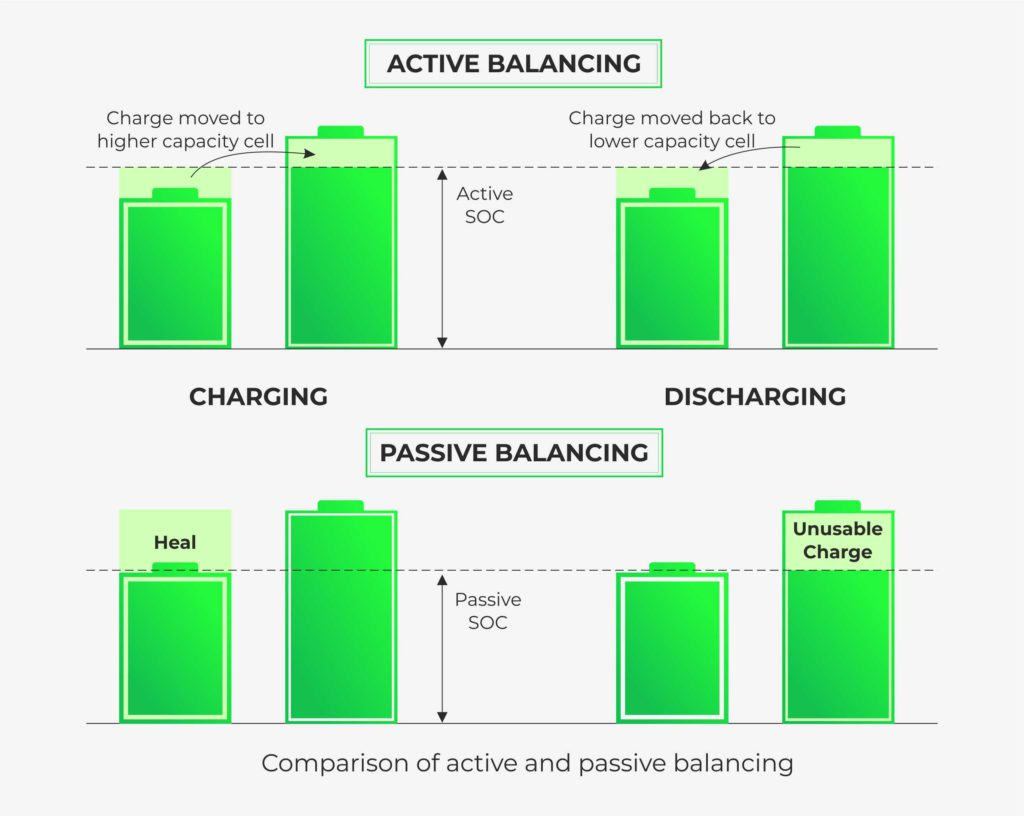
\includegraphics[scale=1.5]{figures/Akku/Vergleichaktivespassives.jpg}
		\caption{Vergleich zwischen Aktiven- und Passiven-Battery Balancing}
	\end{center}
\end{figure}
\newpage

\textbf{Passives Battery-Balancing:}

Eine technische weit verbreitete Methode für das Balancing, ist das Passive Battery-Balancing. Dabei arbeitet es nur im Bereich des Ladeschlusses. Der Ausdruck Ladeschluss bedeutet soviel, dass wenn die Akkumulatoren fast vollständig aufgeladen sind das Balancing zu arbeiten beginnt. Sobald die Zellen die Ladeschlussspannung erreicht haben, wird durch den Balancer ein Widerstand parallel dazugeschalten, um so die Spannung auf die Ladeschlussspannung zu begrenzen. Zellen, welche diese Spannung bereits erreicht haben, werden dann nur noch geringfügig weitergeladen oder teilweise sogar etwas entladen. Die Zellen, die jedoch noch in der Reihenschaltung verschalten sind und die Ladeschlussspannung noch nicht erreicht haben, werden weiterhin mit dem Ladestrom versorgt und somit weitergeladen. Wichtig ist darauf zu achten, dass die Leistung des Parallelwiderstandes auf den Ladstrom angepasst werden muss, da sonst zuviel Energie in Form von Wärme am Widerstand auftreten wird.

\begin{figure}[H]
	\begin{center}
		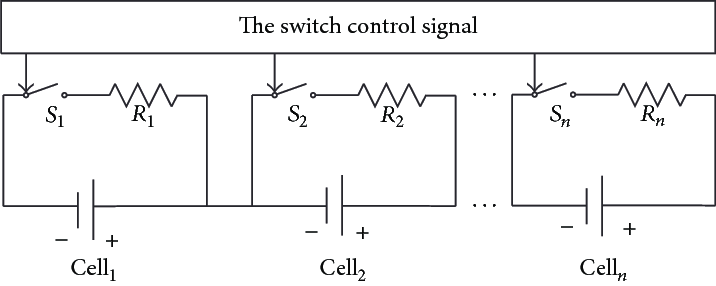
\includegraphics[scale=0.5]{figures/Akku/Passive-cell-balancing.png}
		\caption{Funktionsweise des Passiven Battery-Balancing}
	\end{center}
\end{figure}

\textbf{Vorteile} des Passiven Battery-Balancing:
\begin{itemize}
\item {sehr kostengünsigt} \medskip\\
\item {technisch relativ leicht realisierbar} \medskip\\
\end{itemize}

\textbf{Nachteile} des Passiven Battery-Balancing:
\begin{itemize}
\item {Ladevorgang kann extrem lange dauern, da man warten muss bis die schwächste Zelle den geforderten State of Charge (SOC) erreicht hat} \medskip\\
\item {viel Energie verpufft in Form von Wärme} \medskip\\
\item {Diese Verlustwärme wirkt sich negativ auf die Lebensdauer der Akkumulatoren aus} \medskip\\
\item {nicht unerhebliche Brandgefahr} \medskip\\
\end{itemize}
\newpage

\textbf{Aktives Battery-Balancing:}

Diese Methode des Balancing ist etwas komplexer als beim Passiven Battery-Balancing, jedoch ist sie deutlich effizienter. Bei den aktiven Balancern wird ein Ladungstransfer von Zellen untereinander realisiert. Das bedeutet, dass die Energie der Zellen die bereits ein höher Ladung aufweisen, auf die Akkumulatoren mit niedrigerer Ladung übertragen werden. Beim Aktiven Battery-Balancing werden sogenannte Ladreglungen benötigt. Ladreglungen sind im Prinzip speziell auf eine Anwendung optimierte Schaltregler, die pro Zelle arbeiten und aktiv die Energie übertragen. Dieser Vorgang kann bereits während des Ladeprozesses erfolgen. Standartmäßig wird dieser Vorgang jedoch erst im Bereich des Ladeschlusses aktiv (gleich wie beim Passiven Battery-Balancing). Eine weiterentwickelte Form dieses Systems wird bidirektionalens Balancer-System genannt. Hierbei ist es möglich, dass des Ladungsaustausch sowohl beim Entladen als auch beim Aufladen der Zellen stattfinden kann. Desswegen sind diese bidrektionalen Balancer noch deutlich effizienter. Das Akitve Battery-Balancing wird heutzutage meistens bei größeren Leistungen angewandt, wie zum Beispiel im Bereich der Elektromobilität.

\begin{figure}[H]
	\begin{center}
		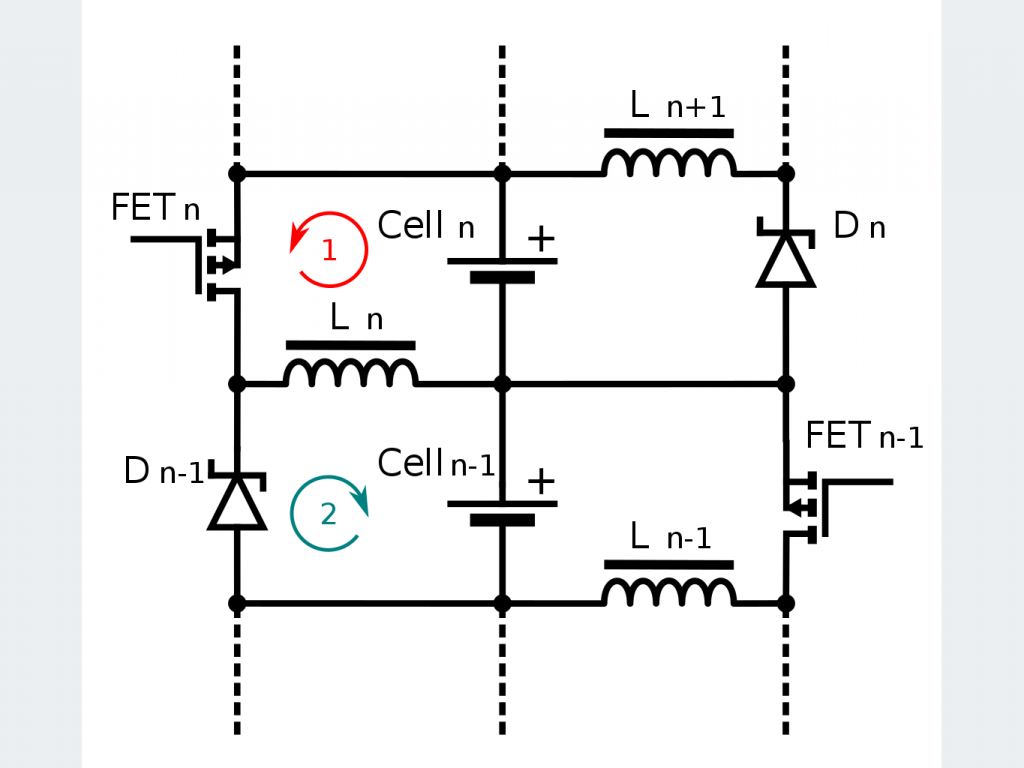
\includegraphics[scale=0.4]{figures/Akku/Aktives Balancing.png}
		\caption{Funktionsweise des Aktiven Battery-Balancing}
	\end{center}
\end{figure}

In der obigen Abbildung kann man die Prinzipschaltung eines aktiven Balancers mit zwei Stufen sehen. Innerhalb von zwei Schaltvorgängen kann dabei die Energie aus der Akkuzelle Cell n über den FET n in die Spule L n übertragen werden (Schleife in rot, 1).
Im zweiten Schaltvorgang (Schleife in blau, 2) wird die Energie in der Spule L n über Diode D n-1 in die Cell n-1 geladen und Cell n-1 aufgeladen.

\textbf{Vorteile} des Aktiven Battery-Balancing:
\begin{itemize}
\item {deutlich höherer Wirkungsgrad als beim passiven Battery-Balancing} \medskip\\
\item {übergeordnete Ladereglung mit intelligenter und lernfähiger Software} \medskip\\
\item {Lebensdauer der Akkumulatoren kann durch die Methode der Ladungsumverteilung deutlich erhöht werden} \medskip\\
\item {überschüssige Energie wird nur zu einem geringen Grad in Wärme umgewandelt} \medskip\\
\item {geringeres Risiko für eine Entflammung} \medskip\\
\end{itemize}

\textbf{Nachteile} des Aktiven Battery-Balancing:
\begin{itemize}
\item {höherer Verschaltungsaufwand, dadurch erhöhte Initialkosten} \medskip\\
\end{itemize}

\section{Steuereinheiten}
\subsection{Raspberry PI}
\section{Bussysteme}
\subsection{SPI Bus}
\subsection{CAN Bus}
